\section{Анализ результатов обучения моделей}

\subsection{Используемые метрики оценки качества}

Задача классификации Bitcoin-адресов является многоклассовой~(6 классов) и несбалансированной. Привычная доля верных предсказаний~(\textit{accuracy}) вводит в заблуждение~--- модель, предсказывающая только мажоритарный класс \textit{miner}, достигнет~43,7\% accuracy при нулевой практической ценности.

Для каждого класса~$c$ вычисляются точность~(\textit{precision}), полнота~(\textit{recall}) и F1-мера:
\begin{equation}\label{eq:f1_class}
    P_c = \frac{TP_c}{TP_c + FP_c}, \quad
    R_c = \frac{TP_c}{TP_c + FN_c}, \quad
    F1_c = \frac{2 P_c R_c}{P_c + R_c},
\end{equation}
где $P_c$~--- точность (precision) для класса~$c$, \\ $R_c$~--- полнота (recall) для класса~$c$, \\ $F1_c$~--- F1-мера для класса~$c$, \\ $TP_c$~--- верно предсказанные образцы класса~$c$, \\ $FP_c$~--- образцы других классов, ошибочно отнесённые к~$c$, \\ $FN_c$~--- образцы класса~$c$, ошибочно отнесённые к другим классам.

\textbf{Взвешенная F1-мера} агрегирует поклассовые F1-меры с весами, пропорциональными числу образцов:
\begin{equation}\label{eq:f1_weighted}
    F1_{\text{weighted}} = \sum_{c=1}^{K} \frac{n_c}{n} F1_c,
\end{equation}
где $K$~--- число классов, \\ $n_c$~--- число образцов класса~$c$ в выборке, \\ $n$~--- общее число образцов, \\ $F1_c$~--- F1-мера класса~$c$.

\textbf{ROC-AUC} в многоклассовой постановке вычисляется по схеме «один против всех»~(OvR): для каждого класса~$c$ строится зависимость~TPR от~FPR при варьировании порога решения. Макро-усреднённый ROC-AUC не учитывает дисбаланс классов:
\begin{equation}\label{eq:roc_auc}
    \text{AUC}_{\text{macro}} = \frac{1}{K} \sum_{c=1}^{K} \text{AUC}_c,
\end{equation}
где $K$~--- число классов, \\ $\text{AUC}_c$~--- площадь под ROC-кривой для класса~$c$ в постановке OvR.

\subsection{Сводные результаты сравнения моделей}

После завершения обучения все шесть моделей оцениваются на отложенной тестовой выборке~(1\,218~адресов). Сводные результаты по двум ключевым метрикам приведены в таблице~\ref{tab:model_comparison} и визуализированы на рисунке~\ref{fig:model_comparison}.

\begin{table}
    \caption{Результаты сравнения моделей на тестовой выборке}
    \begin{tabularx}{\textwidth}{|X|c|c|}
    \hline
    \textbf{Модель} & \textbf{F1-взвешенная} & \textbf{ROC-AUC (макро)} \\
    \hline
    XGBoost & 0,7907 & 0,9610 \\
    \hline
    Stacking & 0,7872 & 0,9517 \\
    \hline
    LightGBM & 0,7830 & 0,9597 \\
    \hline
    Random Forest & 0,7653 & 0,9463 \\
    \hline
    MLP & 0,6614 & 0,9124 \\
    \hline
    kNN & 0,6281 & 0,8769 \\
    \hline
    \end{tabularx}
    \label{tab:model_comparison}
\end{table}

Наилучший результат по обеим метрикам достигнут моделью XGBoost: F1~=~0,7907, AUC~=~0,9610. LightGBM вплотную следует по ROC-AUC~(0,9597), уступая лишь~0,0013. Stacking~(F1~=~0,7872) не превосходит одиночный XGBoost: базовые модели коррелируют в своих ошибках, что ограничивает эффект объединения. MLP~(F1~=~0,6614) уступает методам бустинга на~12,9\% по F1; kNN~(0,6281) демонстрирует наихудший результат из-за «проклятия размерности» в 30-мерном признаковом пространстве. Визуальное сравнение всех шести моделей приведено на рисунке~\ref{fig:model_comparison}.

\begin{figure}
    \centering
    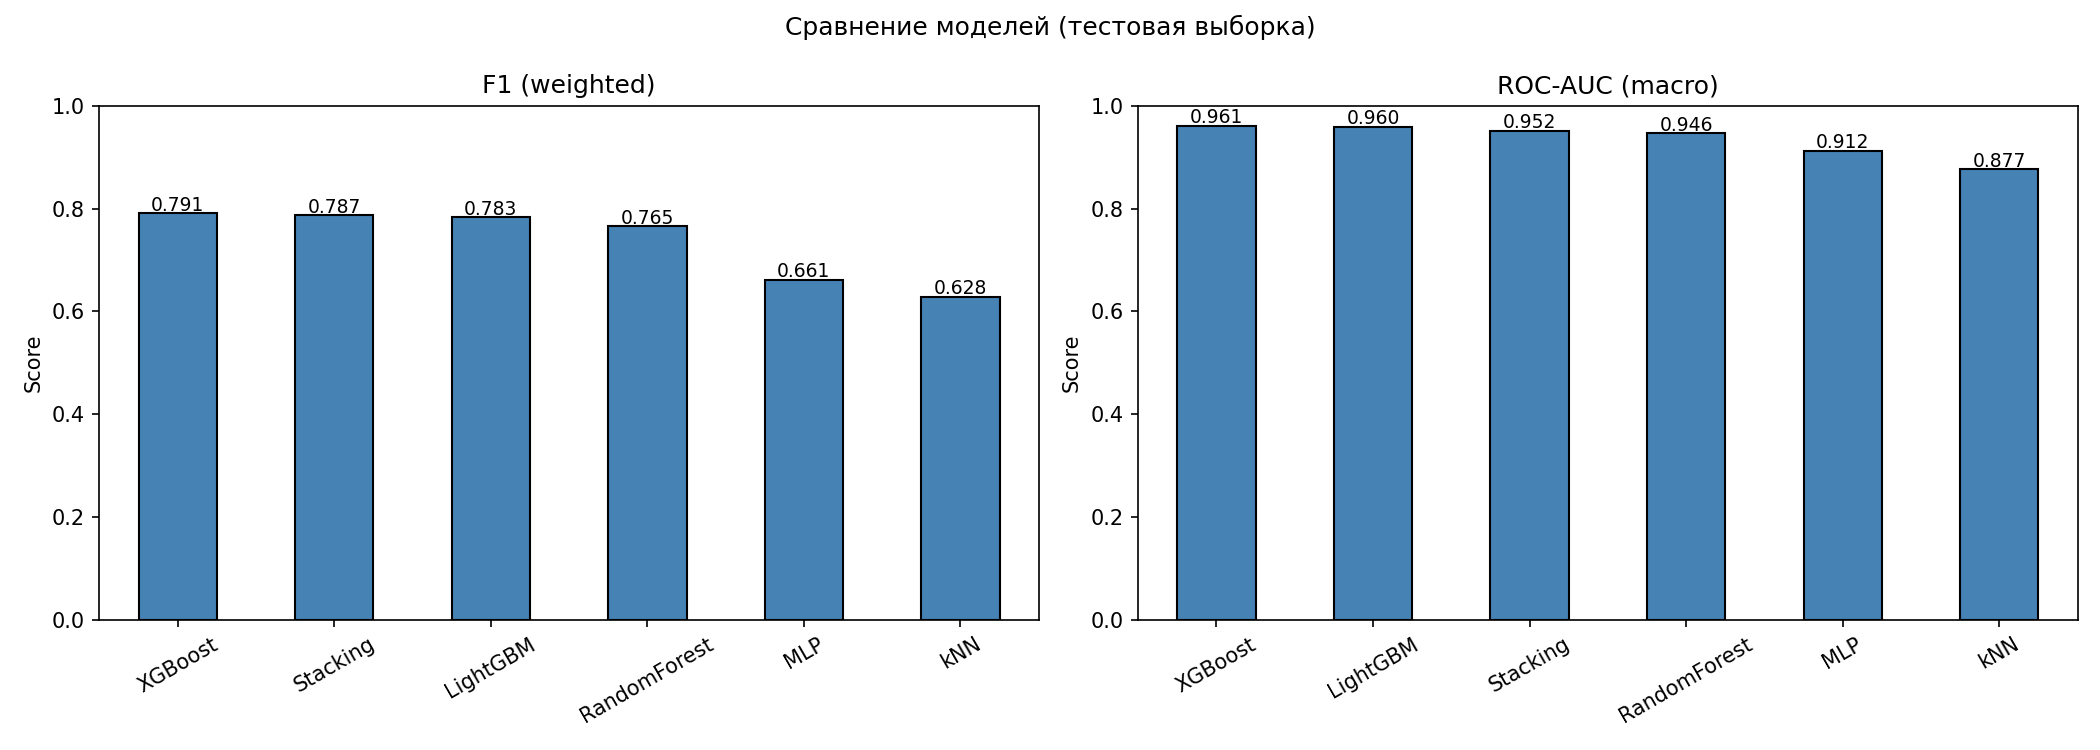
\includegraphics[width=\linewidth]{output/model_comparison.png}
    \caption{Сравнение всех моделей по взвешенной F1-мере~(слева) и макро-усреднённому ROC-AUC~(справа) на тестовой выборке}
    \label{fig:model_comparison}
\end{figure}

\subsection{Матрицы ошибок}

Матрица ошибок нормализована по строкам~--- элемент $M_{ij} = P(\hat{y}=j \mid y=i)$ показывает, с какой вероятностью объект истинного класса~$i$ предсказывается как класс~$j$. Диагональные элементы~$M_{ii}$ равны полноте~(recall) для каждого класса. Цвет ячейки кодирует значение вероятности: более тёмный оттенок соответствует большему значению. Идеальный классификатор имеет единицы на диагонали и нули вне неё; у реального~--- часть вероятностной массы смещена в недиагональные ячейки, отражая ошибки классификации. На рисунках~\ref{fig:cm_xgboost}--\ref{fig:cm_knn} представлены нормализованные матрицы ошибок для всех шести моделей.

\begin{figure}
    \centering
    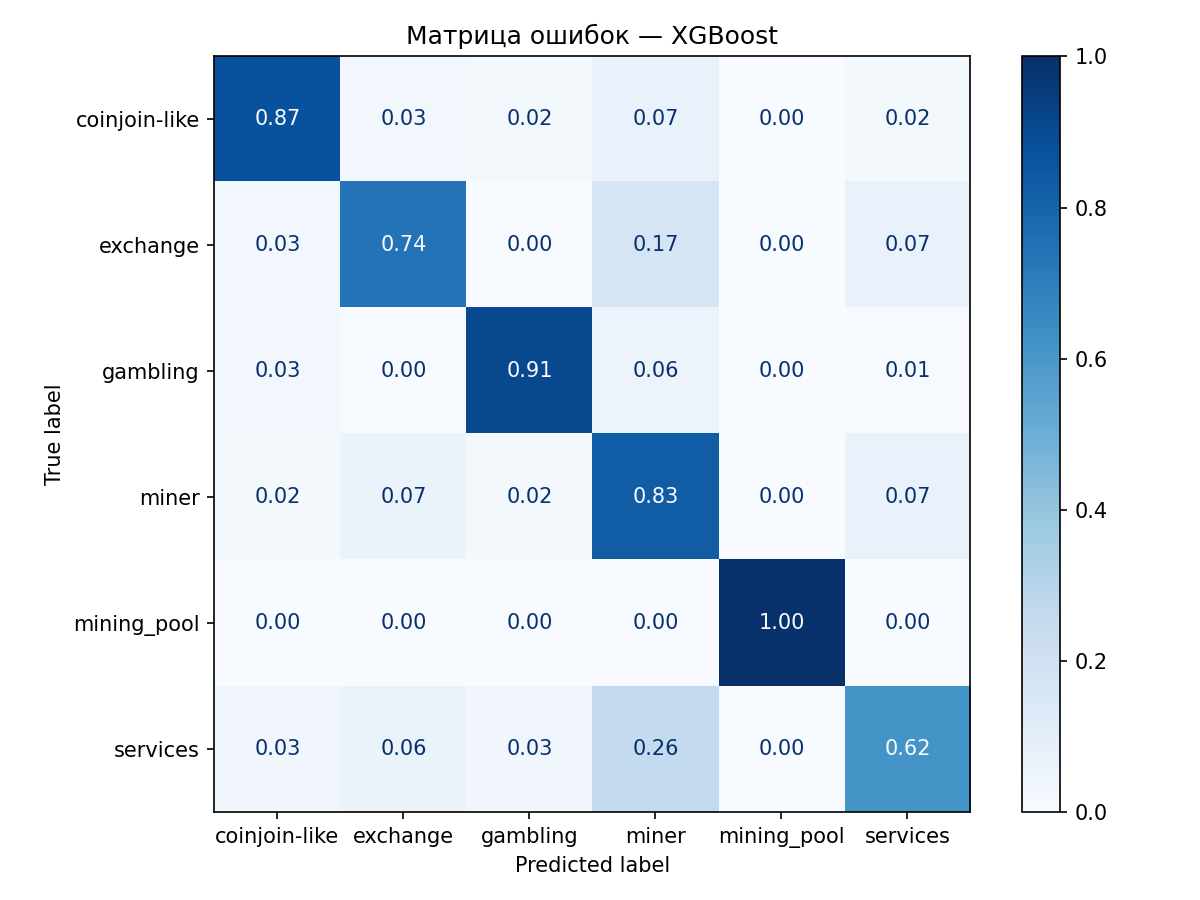
\includegraphics[width=0.82\linewidth]{output/confusion_matrix_XGBoost.png}
    \caption{Нормализованная матрица ошибок модели XGBoost на тестовой выборке}
    \label{fig:cm_xgboost}
\end{figure}

\begin{figure}
    \centering
    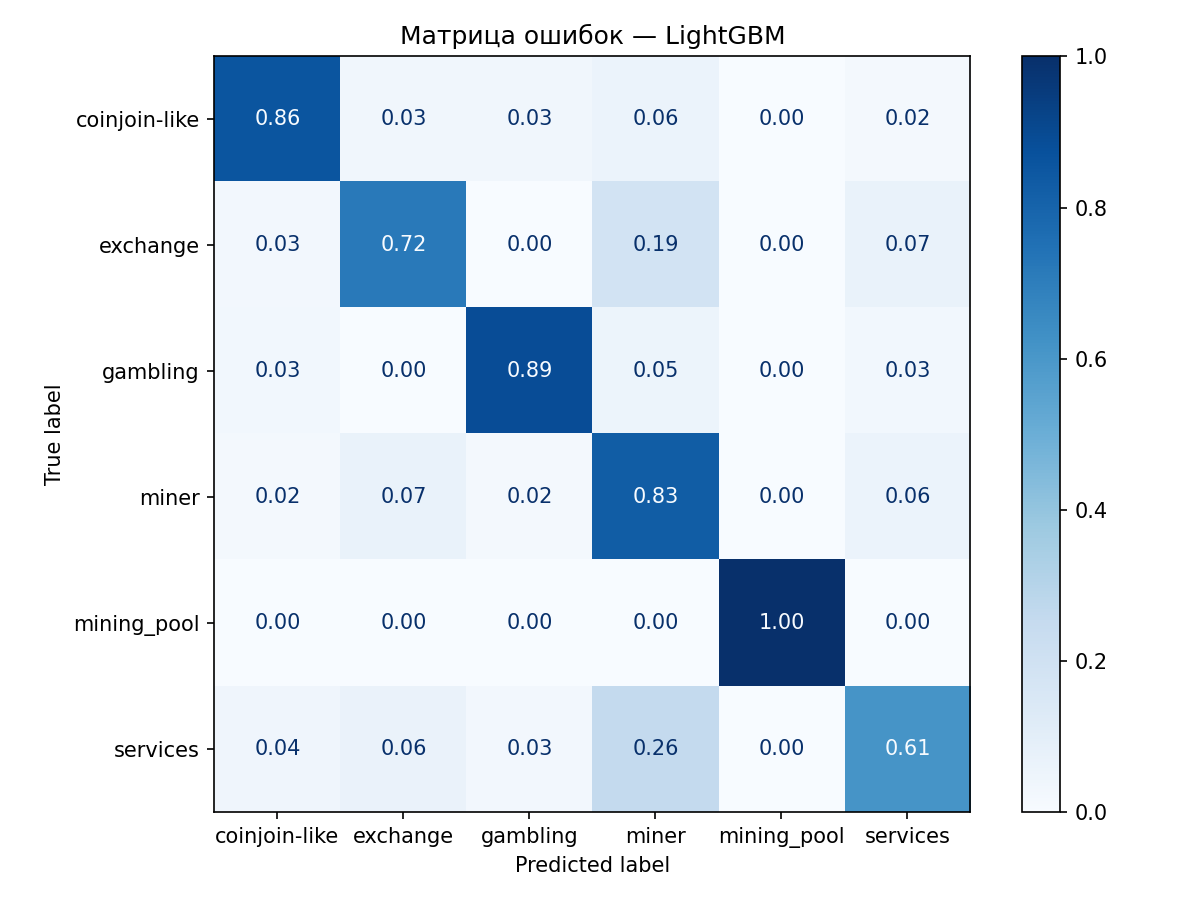
\includegraphics[width=0.82\linewidth]{output/confusion_matrix_LightGBM.png}
    \caption{Нормализованная матрица ошибок модели LightGBM на тестовой выборке}
    \label{fig:cm_lightgbm}
\end{figure}

\begin{figure}
    \centering
    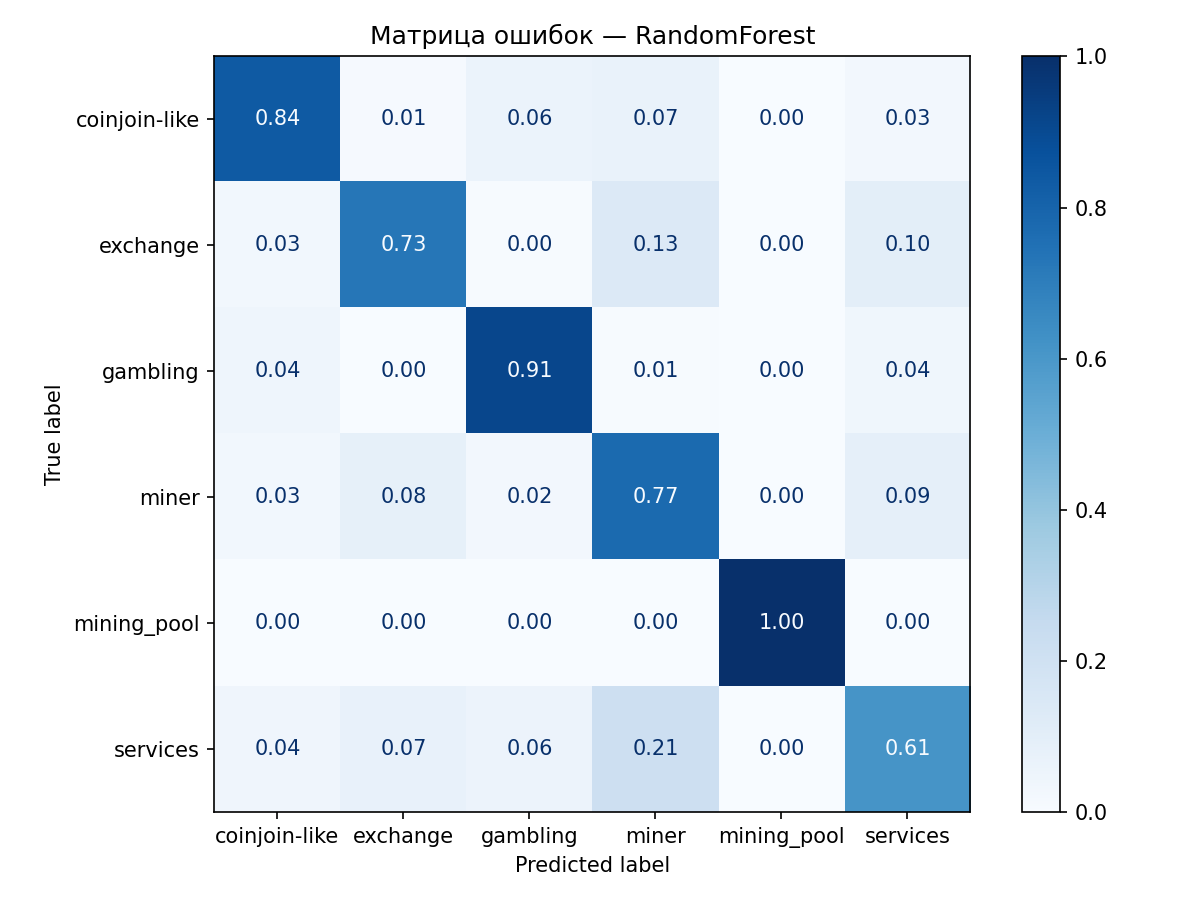
\includegraphics[width=0.82\linewidth]{output/confusion_matrix_RandomForest.png}
    \caption{Нормализованная матрица ошибок модели Random Forest на тестовой выборке}
    \label{fig:cm_rf}
\end{figure}

\begin{figure}
    \centering
    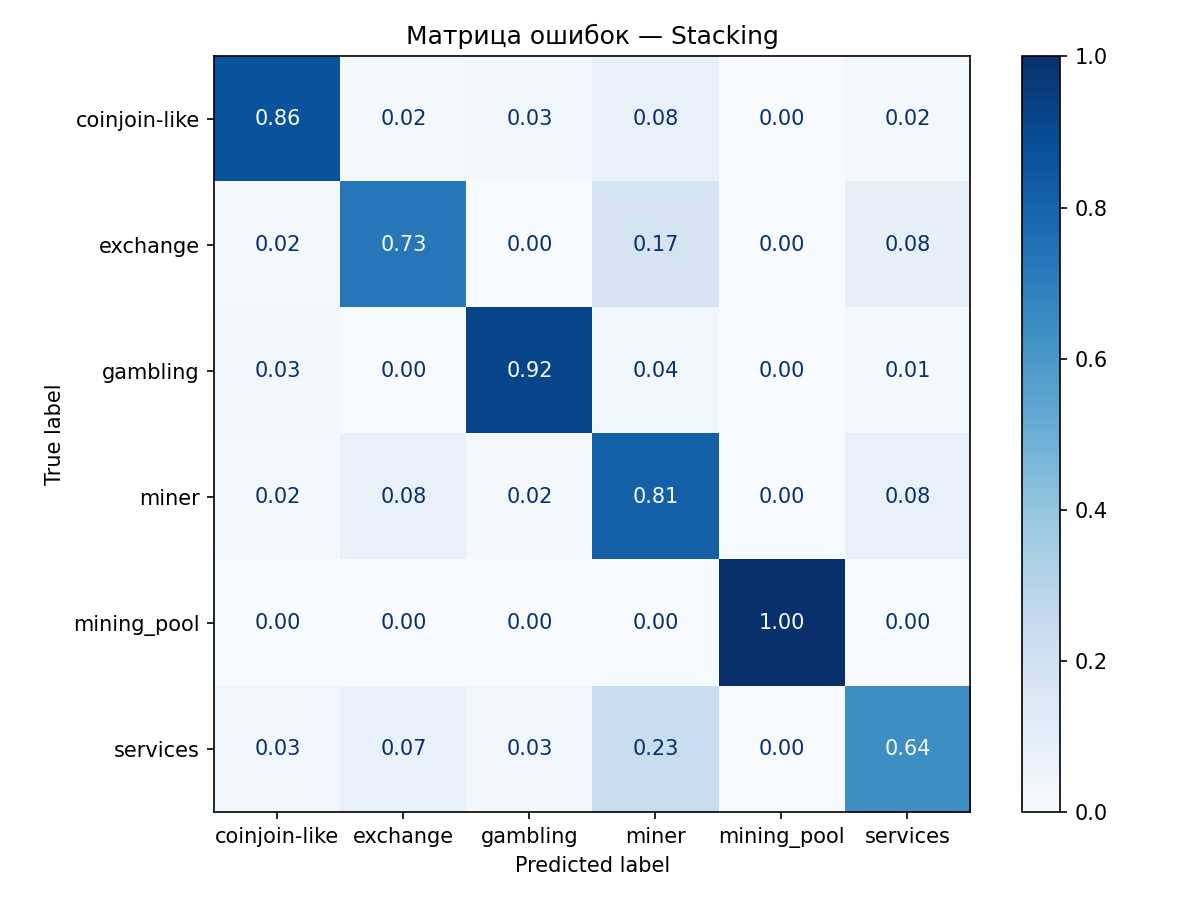
\includegraphics[width=0.82\linewidth]{output/confusion_matrix_Stacking.png}
    \caption{Нормализованная матрица ошибок модели Stacking на тестовой выборке}
    \label{fig:cm_stacking}
\end{figure}

\begin{figure}
    \centering
    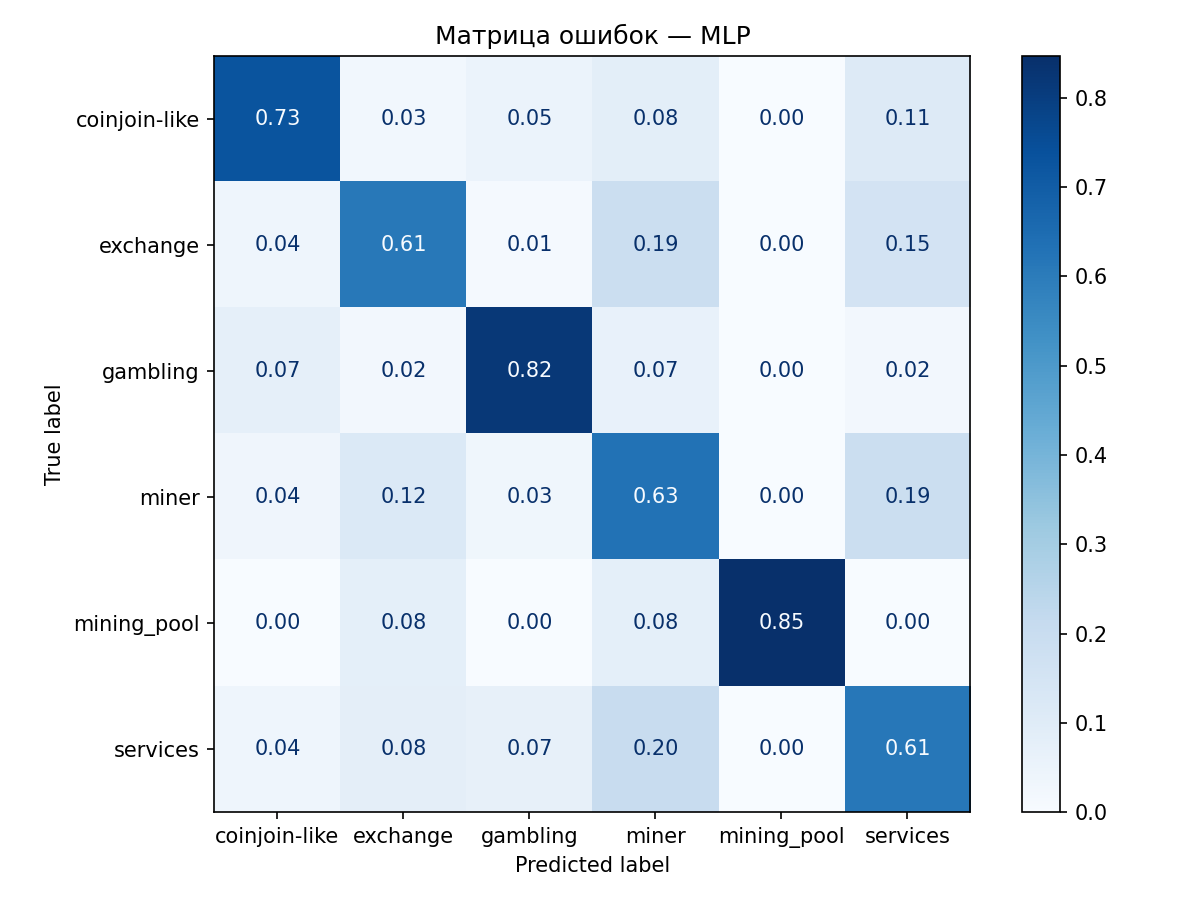
\includegraphics[width=0.82\linewidth]{output/confusion_matrix_MLP.png}
    \caption{Нормализованная матрица ошибок модели MLP на тестовой выборке}
    \label{fig:cm_mlp}
\end{figure}

\begin{figure}
    \centering
    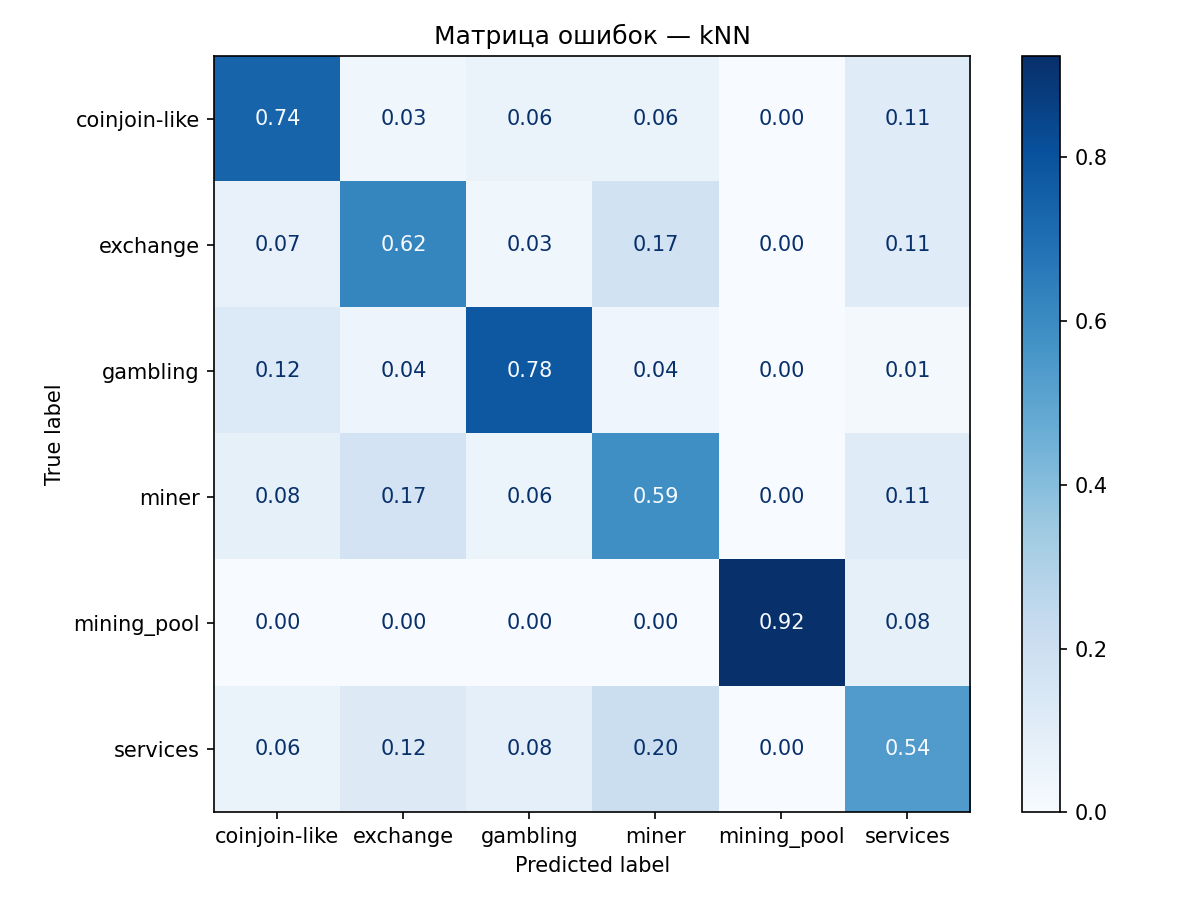
\includegraphics[width=0.82\linewidth]{output/confusion_matrix_kNN.png}
    \caption{Нормализованная матрица ошибок модели kNN на тестовой выборке}
    \label{fig:cm_knn}
\end{figure}

Анализ матриц ошибок~(рисунки~\ref{fig:cm_xgboost}--\ref{fig:cm_knn}) выявляет следующие закономерности. Наибольшую полноту у деревьевидных ансамблей показывают \textit{gambling}~(0,91) и \textit{coinjoin-like}~(0,87) как классы с наиболее характерными транзакционными паттернами; \textit{miner}~(0,83) и \textit{exchange}~(0,74) имеют умеренную полноту несмотря на бо́льшее представление в выборке. Класс \textit{services} устойчиво смешивается с \textit{miner}~--- 20--26\% объектов ошибочно классифицируются как \textit{miner} во всех моделях; у LightGBM~(рисунок~\ref{fig:cm_lightgbm}) доля таких ошибок составляет~26\%, у Random Forest~(рисунок~\ref{fig:cm_rf})~---~21\%. У деревьевидных ансамблей~(рисунки~\ref{fig:cm_xgboost}--\ref{fig:cm_stacking}) \textit{mining\_pool} классифицируется безошибочно~(recall~=~1,00); у MLP~(рисунок~\ref{fig:cm_mlp}) и kNN~(рисунок~\ref{fig:cm_knn}) наблюдается незначительная путаница с \textit{exchange} и \textit{miner}~(по~0,08). Матрицы MLP и kNN значительно более размыты~--- ошибки рассеяны между несколькими классами, что типично для менее мощных классификаторов на небольших табличных данных.

\subsection{ROC-кривые и оптимизация порогов классификации}

\subsubsection{Анализ ROC-кривых}

ROC-кривые построены для каждой модели в постановке OvR~(рисунки~\ref{fig:roc_xgboost}--\ref{fig:roc_knn}). В постановке OvR для шести классов строится шесть независимых бинарных задач: объекты класса~$c$ считаются положительными, все остальные~--- отрицательными; порог решения варьируется от~0 до~1, формируя совокупность пар~$(\text{FPR}_c,\,\text{TPR}_c)$, которые образуют ROC-кривую класса~$c$. Каждая кривая соответствует одному классу: ось~X~--- FPR, ось~Y~--- TPR; в легенде указан AUC для данного класса. Диагональная пунктирная линия соответствует случайному классификатору~(AUC~=~0,5). Площадь под кривой~(AUC) для класса~$c$ численно равна вероятности того, что случайно выбранный объект класса~$c$ получит более высокую оценку принадлежности к~$c$, чем случайно выбранный объект другого класса~--- данная интерпретация делает метрику независимой от порога классификации. Высокий AUC при низкой взвешенной F1 свидетельствует о хорошей ранжирующей способности модели при неоптимальном пороге классификации~0,5; оптимизация порогов по критерию Юдена для лучшей модели рассмотрена в подразделе~2.4.2.

\begin{figure}
    \centering
    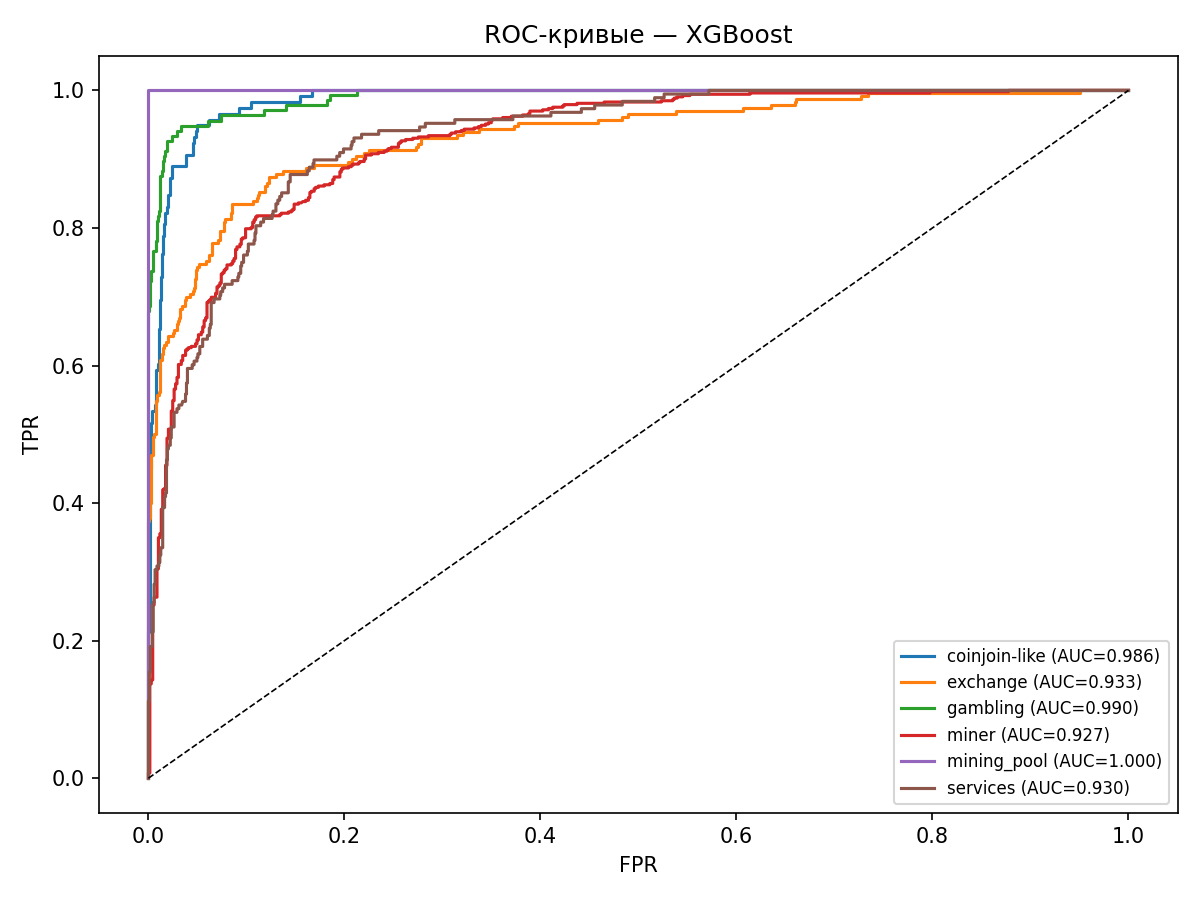
\includegraphics[width=0.82\linewidth]{output/roc_XGBoost.png}
    \caption{ROC-кривые в постановке OvR для модели XGBoost (макро ROC-AUC = 0,9610) на тестовой выборке}
    \label{fig:roc_xgboost}
\end{figure}

\begin{figure}
    \centering
    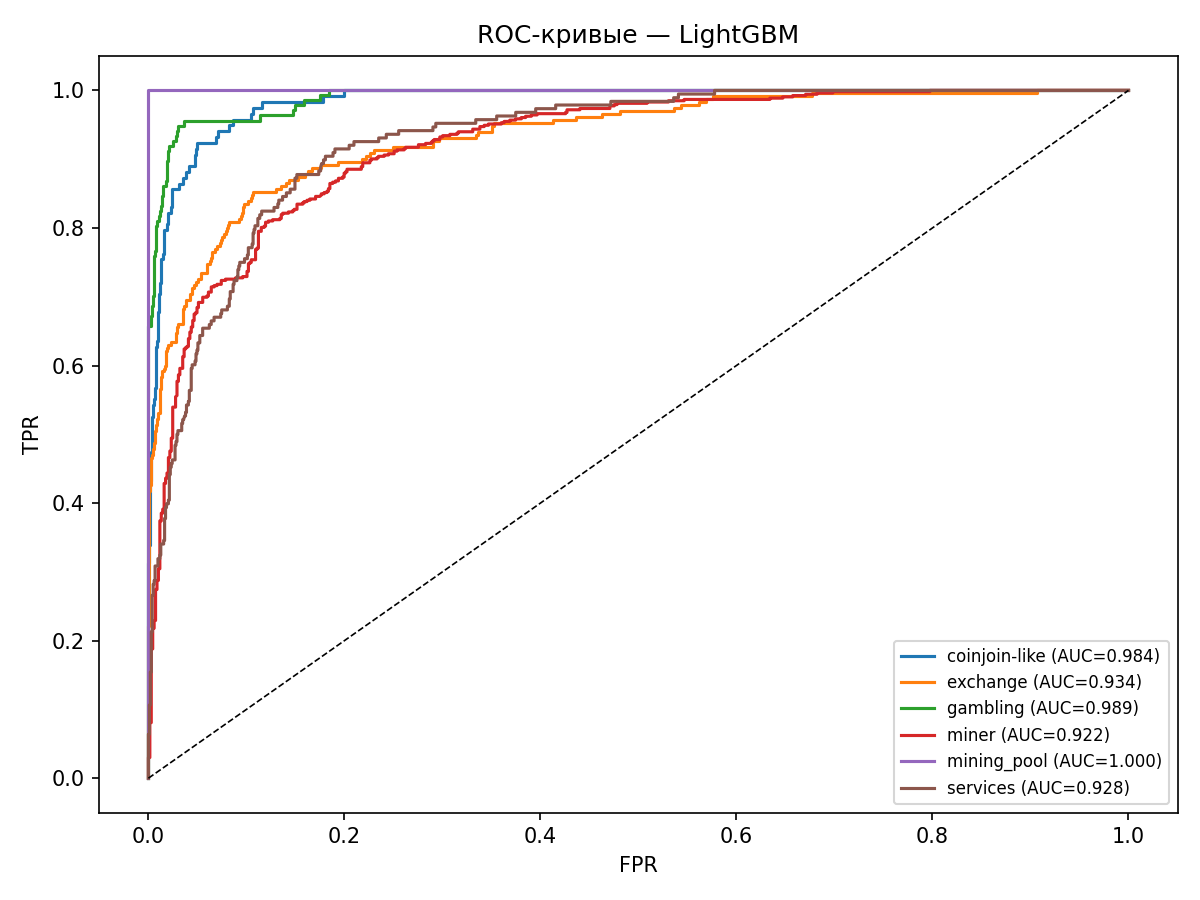
\includegraphics[width=0.82\linewidth]{output/roc_LightGBM.png}
    \caption{ROC-кривые в постановке OvR для модели LightGBM (макро ROC-AUC = 0,9597) на тестовой выборке}
    \label{fig:roc_lightgbm}
\end{figure}

\begin{figure}
    \centering
    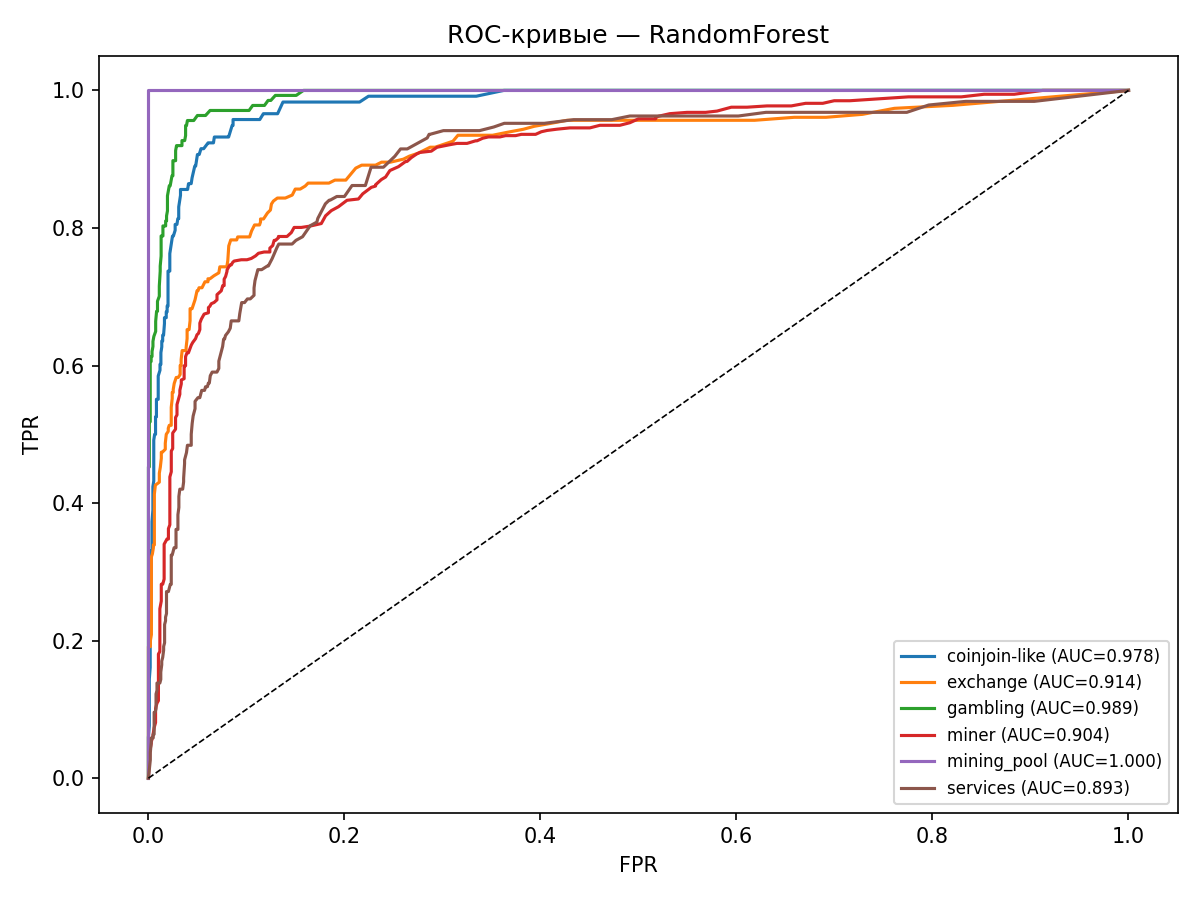
\includegraphics[width=0.82\linewidth]{output/roc_RandomForest.png}
    \caption{ROC-кривые в постановке OvR для Random Forest (макро ROC-AUC = 0,9463) на тестовой выборке}
    \label{fig:roc_rf}
\end{figure}

\begin{figure}
    \centering
    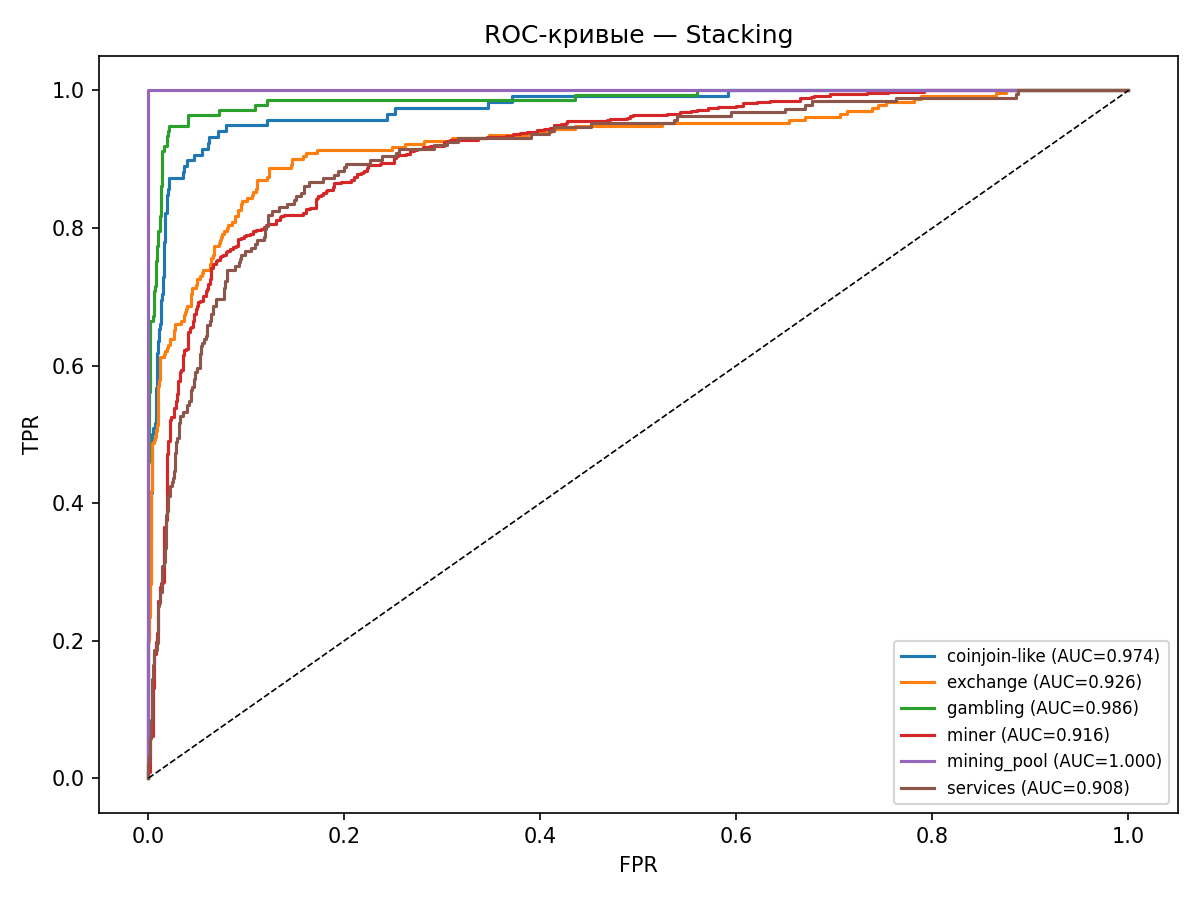
\includegraphics[width=0.82\linewidth]{output/roc_Stacking.png}
    \caption{ROC-кривые в постановке OvR для модели Stacking (макро ROC-AUC = 0,9517) на тестовой выборке}
    \label{fig:roc_stacking}
\end{figure}

\begin{figure}
    \centering
    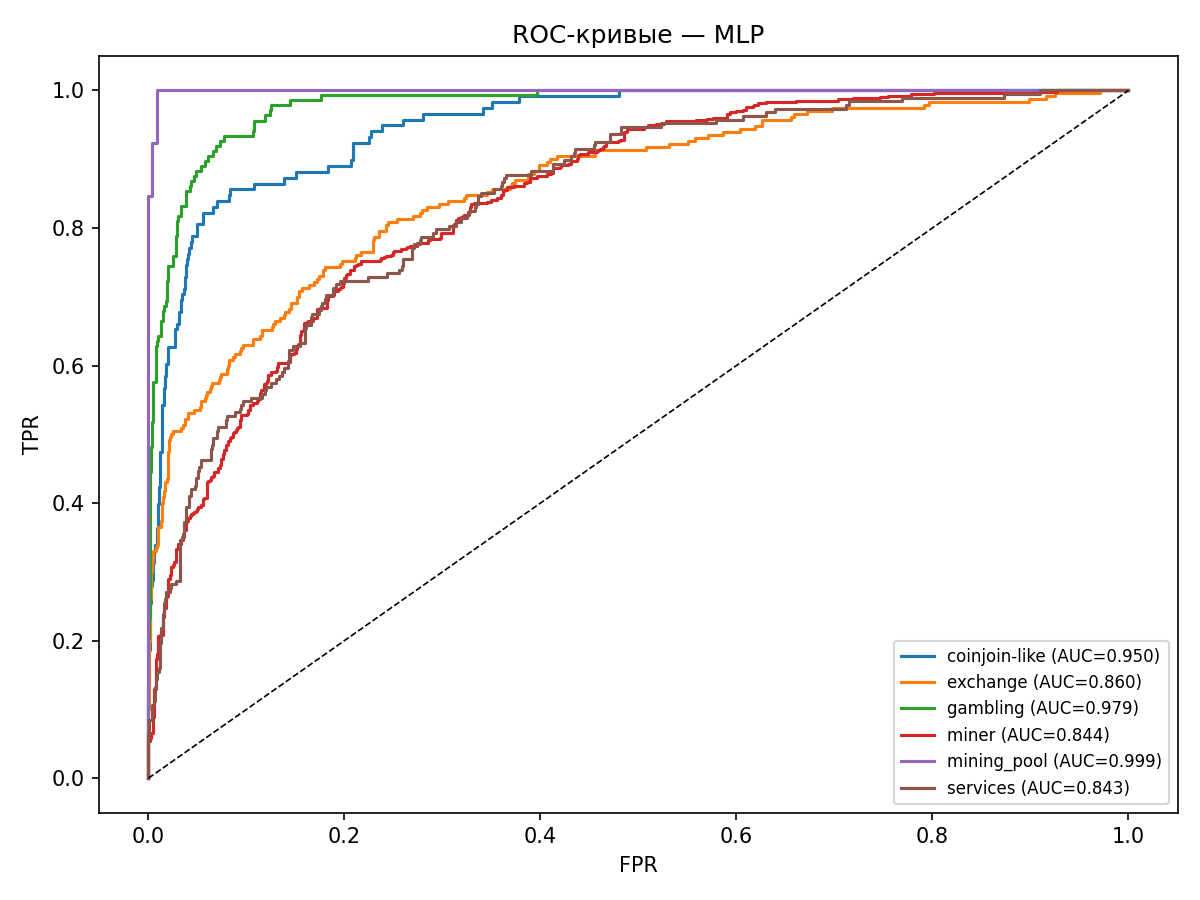
\includegraphics[width=0.82\linewidth]{output/roc_MLP.png}
    \caption{ROC-кривые в постановке OvR для модели MLP (макро ROC-AUC = 0,9124) на тестовой выборке}
    \label{fig:roc_mlp}
\end{figure}

\begin{figure}
    \centering
    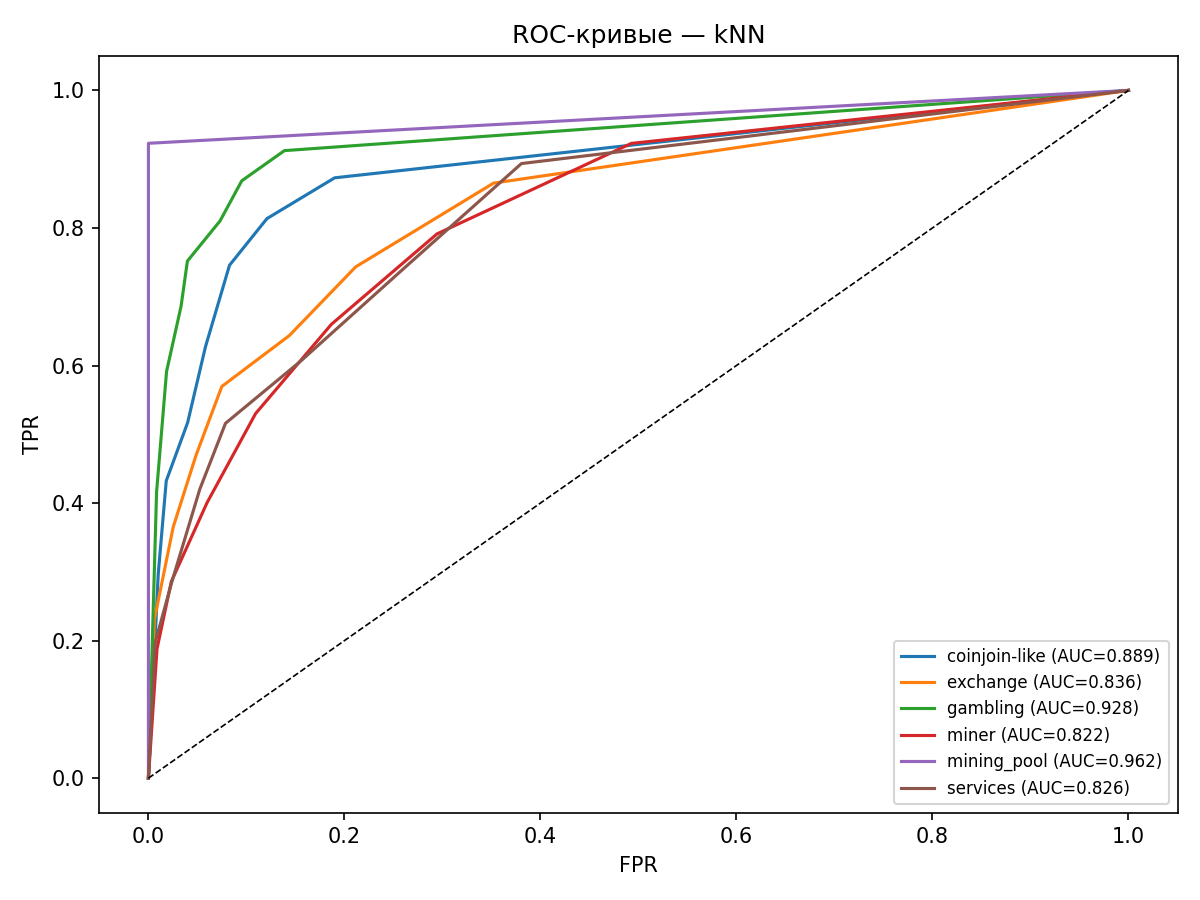
\includegraphics[width=0.82\linewidth]{output/roc_kNN.png}
    \caption{ROC-кривые в постановке OvR для модели kNN (макро ROC-AUC = 0,8769) на тестовой выборке}
    \label{fig:roc_knn}
\end{figure}

ROC-кривые XGBoost~(рисунок~\ref{fig:roc_xgboost}) и LightGBM~(рисунок~\ref{fig:roc_lightgbm}) демонстрируют крутой подъём в левой части: высокий TPR достигается при малом FPR, что отвечает требованиям~AML-систем. Stacking~(рисунок~\ref{fig:roc_stacking}) незначительно превосходит Random Forest~(рисунок~\ref{fig:roc_rf}) по AUC. Для MLP~(рисунок~\ref{fig:roc_mlp}) кривые ниже, чем у деревьевидных ансамблей, что отражает меньшую разделимость классов. Для kNN~(рисунок~\ref{fig:roc_knn}) кривые заметно ниже и менее упорядочены~--- метод не формирует хорошо калиброванных вероятностей в высокодимензиональном пространстве. Наименьший AUC во всех моделях~--- у класса~\textit{services}.

\subsubsection{Критерий Юдена и оптимизация порогов}

Для лучшей модели~(XGBoost) выполнена оптимизация порогов по критерию Юдена. Для класса~$c$ оптимальный порог определяется как $\tau_c^* = \arg\max_{\tau} J_c(\tau)$, где $J_c(\tau) = \text{TPR}_c(\tau) - \text{FPR}_c(\tau)$~--- статистика Юдена; $\text{TPR}_c(\tau)$~--- чувствительность (доля верно выявленных объектов класса~$c$) при пороге~$\tau$; $\text{FPR}_c(\tau)$~--- доля ложных тревог при пороге~$\tau$.
Итоговый класс: $\hat{y} = \arg\max_c (p_c(\mathbf{x}) - \tau_c^*)$. Оптимальные пороги оказываются ниже~0,5 для миноритарных классов~(\textit{mining\_pool},~\textit{coinjoin-like}), повышая их полноту. Взвешенная F1 при оптимизации~--- 0,7844~--- незначительно ниже исходных~0,7907: повышение полноты миноритарных классов сопровождается снижением точности мажоритарных, что незначительно снижает взвешенный агрегат, но важно для~AML-задач.

\subsection{Интерпретация предсказаний методом SHAP}

Метод~\acrshort{shap}~\cite{shap_paper} позволяет объяснить любое предсказание через значения Шепли из теории игр~--- справедливое распределение вклада каждого признака:
\begin{equation}\label{eq:shap}
    \phi_j = \sum_{S \subseteq \mathcal{F} \setminus \{j\}} \frac{|S|!\,(|\mathcal{F}|-|S|-1)!}{|\mathcal{F}|!}
    \bigl[f(\mathbf{x}_{S \cup \{j\}}) - f(\mathbf{x}_S)\bigr], \quad \sum_j \phi_j = f(\mathbf{x}) - \mathbb{E}[f],
\end{equation}
где $\phi_j$~--- значение Шепли признака~$j$, отражающее его вклад в конкретное предсказание, \\ $\mathcal{F}$~--- полное множество признаков, \\ $S \subseteq \mathcal{F} \setminus \{j\}$~--- подмножество признаков без~$j$, \\ $f(\mathbf{x}_{S \cup \{j\}})$~--- предсказание модели при наличии признаков из $S \cup \{j\}$, \\ $f(\mathbf{x}_S)$~--- предсказание без признака~$j$, \\ $\mathbb{E}[f]$~--- среднее предсказание по всей выборке.

Для XGBoost применён \textit{TreeExplainer}~--- точный полиномиальный алгоритм для ансамблей деревьев. Для MLP~--- \textit{PermutationExplainer} с~50~фоновыми образцами, использующий апроксимацию перестановками.

На рисунках~\ref{fig:shap_xgboost} и~\ref{fig:shap_mlp} представлены \textit{beeswarm}-диаграммы для XGBoost и MLP. Каждая точка~--- один объект тестовой выборки; горизонтальная ось~--- значение~SHAP (положительное сдвигает предсказание в сторону данного класса); цвет~--- исходное значение признака~(красный~--- высокое, синий~--- низкое).

\begin{figure}
    \centering
    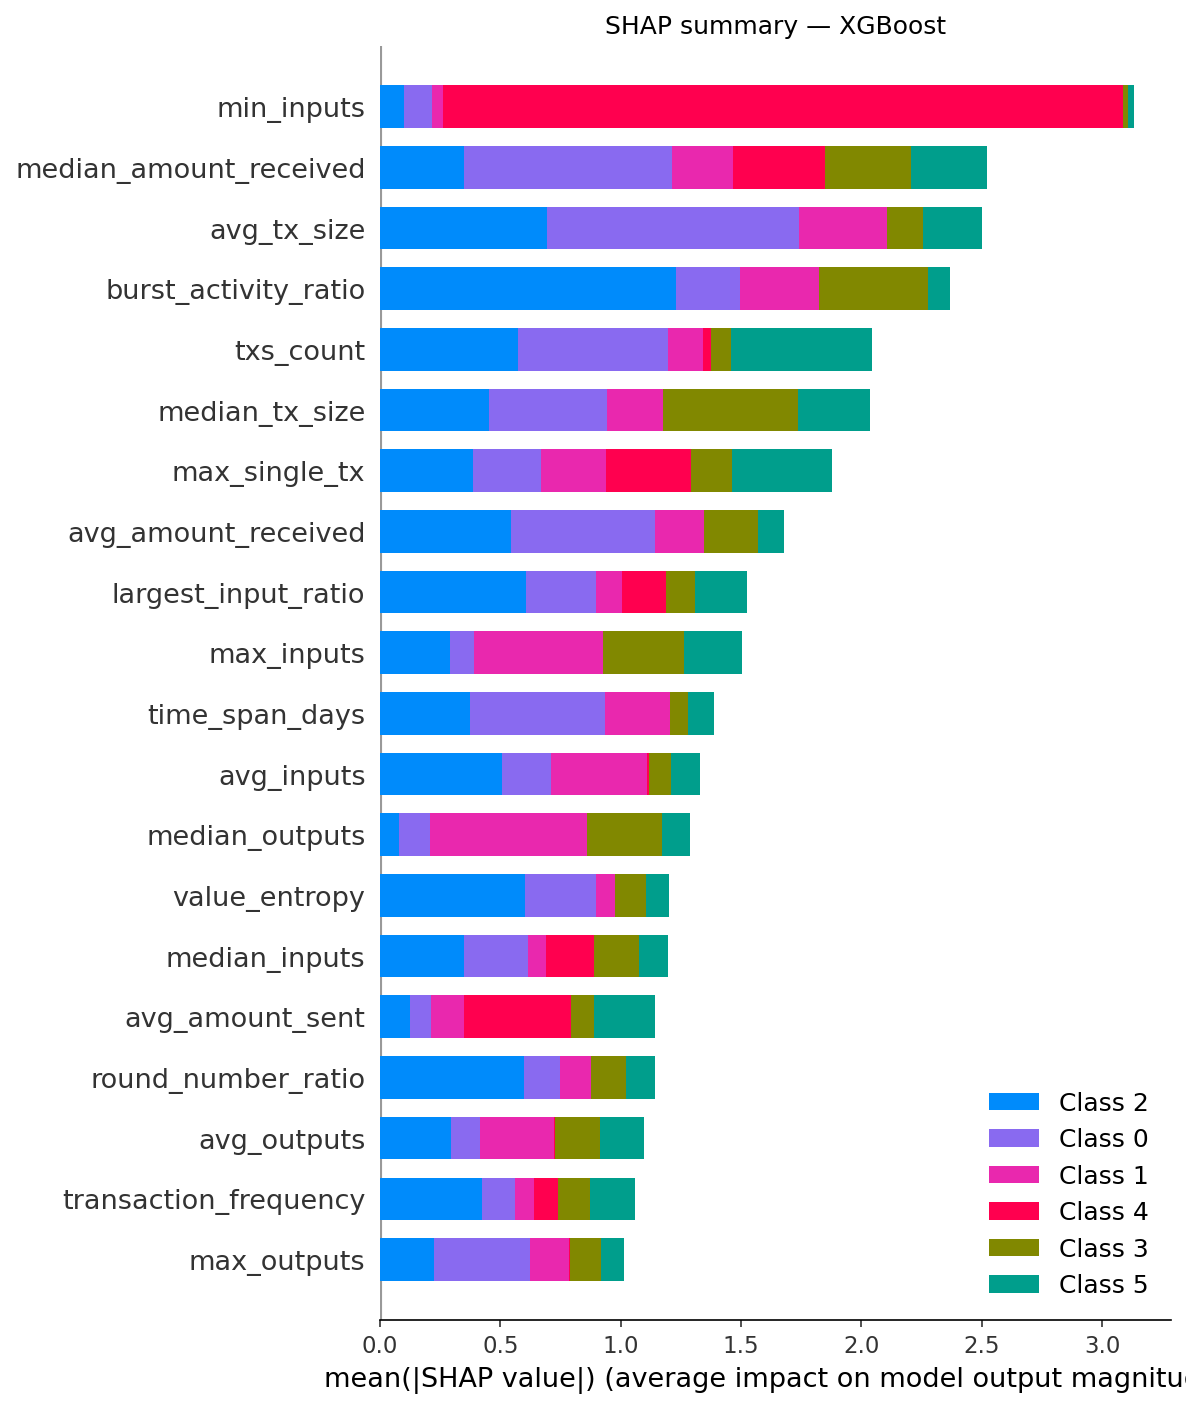
\includegraphics[width=\linewidth]{output/shap_summary_XGBoost.png}
    \caption{SHAP-диаграмма (\textit{beeswarm}) для модели XGBoost, построенная методом \textit{TreeExplainer}}
    \label{fig:shap_xgboost}
\end{figure}

\begin{figure}
    \centering
    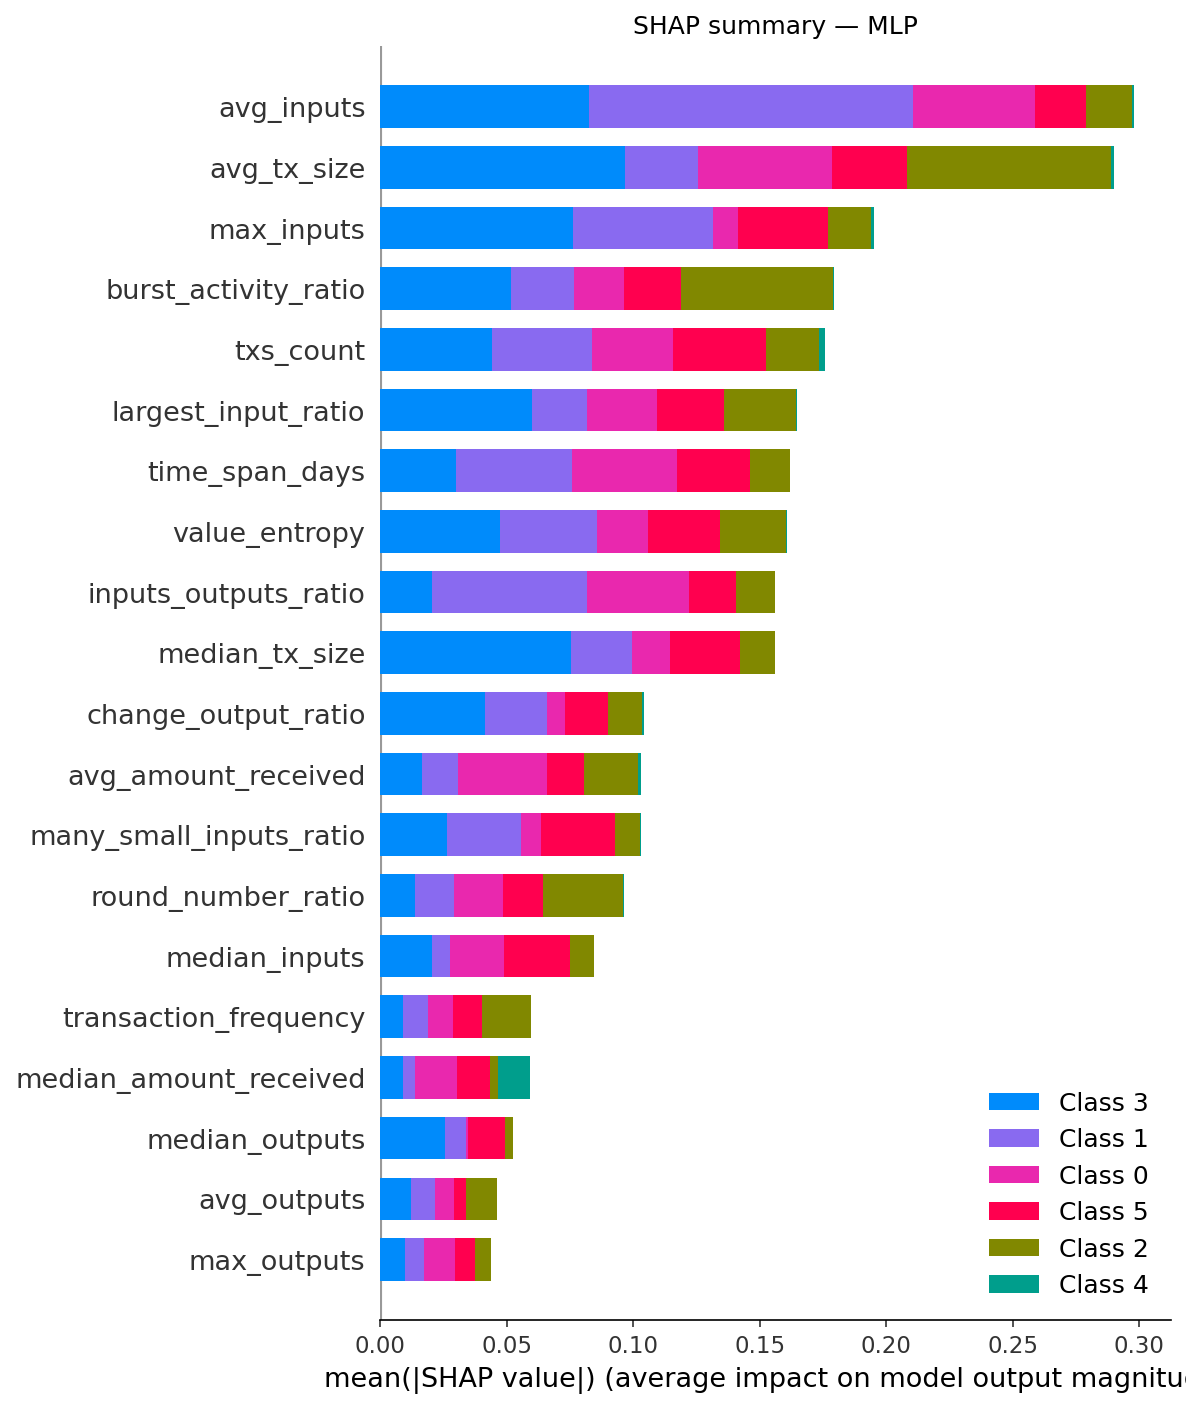
\includegraphics[width=\linewidth]{output/shap_summary_MLP.png}
    \caption{SHAP-диаграмма (\textit{beeswarm}) для модели MLP, построенная методом \textit{PermutationExplainer} с~50~фоновыми образцами}
    \label{fig:shap_mlp}
\end{figure}

По SHAP-диаграмме XGBoost~(рисунок~\ref{fig:shap_xgboost}) наибольший вклад вносят:
\begin{itemize}
    \item \textit{временны́е признаки}~--- среднее время между транзакциями и период активности: майнеры работают непрерывно с коротким ритмом, биржи~--- равномерно круглосуточно;
    \item \textit{экономические признаки}~--- средний объём и суммарный оборот: биржи обрабатывают на порядки больше, чем игровые адреса;
    \item \textit{структурные признаки}~--- число уникальных контрагентов, fan-out: пулы имеют много плательщиков, индивидуальные майнеры~--- мало;
    \item \textit{Bitcoin-специфичные}~--- SegWit, UTXO-паттерны: умеренный вклад, помогают идентифицировать~\textit{coinjoin-like}.
\end{itemize}

Рейтинг по SHAP совпадает с корреляционным анализом~НИРС-02 для топ-10 признаков~--- зависимости воспроизводимы. SHAP-диаграмма MLP~(рисунок~\ref{fig:shap_mlp}) показывает схожий порядок, однако значения распределены равномернее: XGBoost фокусируется на ключевых признаках точнее.

\subsection{Сравнительный анализ моделей}

Результаты подтверждают преимущество деревьевидных ансамблей над нейросетями на табличных данных~\cite{tabular_dl_survey}. Основные причины:
\begin{itemize}
    \item \textit{Явные условные зависимости}: деревья моделируют правила «если $x_j > t$ и $x_k < s$, то класс~$c$» напрямую; MLP аппроксимирует их через нелинейные комбинации весов, что требует больше параметров и данных.
    \item \textit{Инвариантность к распределению}: пороговые разбиения деревьев не зависят от формы распределения признаков; MLP чувствителен к скошенности даже после стандартизации.
    \item \textit{Объём данных}: 14\,892 образца недостаточно, чтобы реализовать потенциал MLP с архитектурой 256-128-64; регуляризация лишь частично компенсирует дефицит.
\end{itemize}

Stacking не превосходит XGBoost~--- базовые модели~(Random Forest, XGBoost и LightGBM) принадлежат одному классу методов и коррелируют в своих ошибках. Эффективнее было бы объединение XGBoost и MLP как принципиально разных подходов.

\subsection{Анализ проблемных классов}

Класс~\textit{services}~--- наиболее сложный: F1~$\approx$~0,65 у XGBoost, $\approx$~0,55 у MLP. Причины: неоднородный состав класса~(платёжные процессоры, миксеры, кошельковые сервисы); пересечение с~\textit{miner} по структурным признакам~--- в частности, по числу и минимальному размеру входов транзакций~(признак~\textit{min\_inputs} наиболее значим по SHAP); в тестовой выборке~187 объектов~--- оценка нестабильна. Рекомендации: детальная перемаркировка с разбиением на подкатегории, извлечение графовых признаков~(центральность, кластерный коэффициент), сбор дополнительных примеров.
